%=========================================================
% SEMINAR REPORT
% ENHANCING PHISHING DETECTION
%=========================================================

\documentclass[12pt,a4paper]{report}
\usepackage[T1]{fontenc}
\usepackage[utf8]{inputenc}

%=========================================================
% PACKAGES
%=========================================================

\usepackage[a4paper,
            top=1in,
            bottom=1in,
            left=1.3in,
            right=1in]{geometry}

% PDFLaTeX-compatible Times-style font
% Use XeLaTeX/LuaLaTeX only if you specifically need a system font.
\usepackage{newtxtext}
\usepackage{newtxmath}

\usepackage{graphicx}
\usepackage{fancyhdr}
\usepackage{titlesec}
\usepackage{tocloft}
\usepackage{setspace}
\usepackage{amsmath,amssymb}
\usepackage{enumitem}
\usepackage{hyperref}
\usepackage{booktabs}
\usepackage{array}
\usepackage{caption}
\usepackage{xcolor}
\usepackage{float}
\usepackage{ragged2e}
\usepackage[nottoc]{tocbibind}
\usepackage{longtable}

%=========================================================
% HYPERLINK SETTINGS
%=========================================================

\hypersetup{
    colorlinks=true,
    linkcolor=black,
    citecolor=black,
    urlcolor=blue,
    pdftitle={ENHANCING PHISHING DETECTION: A MACHINE LEARNING APPROACH WITH FEATURE SELECTION AND DEEP LEARNING MODELS},
    pdfauthor={Ansaf Shan}
}

%=========================================================
% GENERAL FORMATTING
%=========================================================

\onehalfspacing
\fontsize{12}{18}\selectfont

\setlength{\parindent}{0.5in}
\setlength{\parskip}{0pt}

%=========================================================
% CHAPTER FORMATTING
%=========================================================

\titleformat{\chapter}[display]
    {\normalfont\fontsize{16}{19}\selectfont\bfseries\centering}
    {\chaptertitlename\ \thechapter}
    {14pt}
    {\fontsize{16}{19}\selectfont\centering}

\titlespacing*{\chapter}
    {0pt}
    {-8pt}
    {14pt}

%=========================================================
% SECTION FORMATTING (UPDATED TO EXACT 14PT)
%=========================================================

\titleformat{\section}
    {\normalfont\fontsize{14}{17}\selectfont\bfseries}
    {\thesection}
    {0.5em}
    {}

\titleformat{\subsection}
    {\normalfont\fontsize{14}{17}\selectfont\bfseries}
    {\thesubsection}
    {0.5em}
    {}

%=========================================================
% TABLE OF CONTENTS FORMATTING
%=========================================================

\setlength{\cftbeforechapskip}{10pt}
\setlength{\cftbeforesecskip}{4pt}

\renewcommand{\cftchapfont}{\fontsize{12}{14}\selectfont\bfseries}
\renewcommand{\cftsecfont}{\fontsize{12}{14}\selectfont}

\renewcommand{\cftchappagefont}{\fontsize{12}{14}\selectfont\bfseries}
\renewcommand{\cftsecpagefont}{\fontsize{12}{14}\selectfont}

\renewcommand{\cfttoctitlefont}
    {\hfill\fontsize{14}{17}\selectfont\bfseries}

\renewcommand{\cftaftertoctitle}
    {\hfill}

%=========================================================
% HEADER AND FOOTER
%=========================================================

\pagestyle{fancy}

\fancyhf{}

\fancyhead[L]{
    \footnotesize College of Engineering, Cherthala
}

\fancyhead[R]{
    \footnotesize\leftmark
}

\fancyfoot[L]{
    \small Department of Computer Science and Engineering
}

\fancyfoot[R]{
    \small\thepage
}

\renewcommand{\headrulewidth}{0.4pt}
\renewcommand{\footrulewidth}{0.4pt}

\renewcommand{\chaptermark}[1]{
    \markboth{#1}{}
}

%=========================================================
% PLAIN PAGE STYLE
%=========================================================

\fancypagestyle{plain}{
    \fancyhf{}

    \fancyfoot[L]{
        \small Department of Computer Science and Engineering
    }

    \fancyfoot[R]{
        \small\thepage
    }

    \renewcommand{\headrulewidth}{0pt}
    \renewcommand{\footrulewidth}{0.4pt}
}

%=========================================================
% FIGURE CAPTION FORMAT
%=========================================================

\captionsetup[figure]{
    font=normalsize,
    labelfont=normalfont,
    justification=centering,
    singlelinecheck=true
}

\captionsetup[table]{
    font=normalsize,
    labelfont=bf,
    justification=centering,
    singlelinecheck=true
}

%=========================================================
% DOCUMENT INFORMATION
%=========================================================

\newcommand{\reporttitle}{ENHANCING PHISHING DETECTION: A MACHINE LEARNING APPROACH WITH FEATURE SELECTION AND DEEP LEARNING MODELS}
\newcommand{\studentname}{ANSAF SHAN}
\newcommand{\rollno}{CEC23CS038}
\newcommand{\guidename}{Mrs. Fathima N}
\newcommand{\seminarmonth}{AUGUST 2026}
\newcommand{\coordinator}{Mrs. Deepa C G}
\newcommand{\hodname}{Dr. Preetha Theresa Joy}
\newcommand{\principalname}{Dr. Jaya VL}
%=========================================================
% DOCUMENT
%=========================================================

\begin{document}

%=========================================================
% COVER PAGE
%=========================================================

\begin{titlepage}
\thispagestyle{empty}
\begin{center}

\vspace*{0.3cm}

{\Large\bfseries A SEMINAR REPORT ON}\par

\vspace{0.5cm}

{\fontsize{18}{22}\selectfont\bfseries
ENHANCING PHISHING DETECTION:\\
A MACHINE LEARNING APPROACH WITH FEATURE SELECTION\\
AND DEEP LEARNING MODELS}\par

\vfill

{\large\itshape Submitted By}\par
\vspace{0.2cm}
{\large\bfseries\itshape \studentname (\rollno)}\par

\vfill

{\large\itshape under the esteemed guidance of}\par
\vspace{0.2cm}
{\large\bfseries\itshape \guidename}\par
\vspace{0.1cm}
{\large\itshape (Assistant Professor)}\par
\vspace{0.15cm}
{\large\itshape Department of Computer Science and Engineering}\par

\vfill


\includegraphics[width=3.2cm]{logo.jpg}\par

\vfill

{\large\bfseries \seminarmonth}\par
\vspace{0.05cm}
{\large\bfseries DEPARTMENT OF COMPUTER SCIENCE AND ENGINEERING}\par
{\large\bfseries COLLEGE OF ENGINEERING, PALLIPPURAM P O, CHERTHALA,}\par
{\large\bfseries ALAPPUZHA PIN: 688541,}\par
{\large\bfseries PHONE: 0478 2553416, FAX: 0478 2552714}\par
{\large\bfseries http://www.cectl.ac.in}\par

\vspace*{0.3cm}
\end{center}
\end{titlepage}

% =========================================================
% SECOND TITLE PAGE
% =========================================================

\begin{titlepage}
\thispagestyle{empty}
\begin{center}

\vspace*{0.2cm}

{\Large\bfseries A SEMINAR REPORT ON}\par

\vspace{0.45cm}

{\fontsize{17}{21}\selectfont\bfseries
ENHANCING PHISHING DETECTION:\\
A MACHINE LEARNING APPROACH WITH FEATURE SELECTION\\
AND DEEP LEARNING MODELS}\par

\vspace{0.55cm}

{\large\itshape Submitted By}\par
\vspace{0.2cm}
{\large\bfseries\itshape \studentname (\rollno)}\par

\vspace{0.4cm}

{\large\itshape under the esteemed guidance of}\par
\vspace{0.2cm}
{\large\bfseries\itshape \guidename}\par
\vspace{0.1cm}
{\large\itshape (Assistant Professor)}\par

\vspace{0.4cm}

{\large\itshape In partial fulfillment of the requirements for the award of the degree}\par
{\large\itshape of}\par
{\large\bfseries Bachelor of Technology}\par
{\large\itshape in}\par
{\large\bfseries Computer Science and Engineering}\par
{\large\itshape of}\par
{\large\bfseries APJ Abdul Kalam Technological University}\par

\vfill


\includegraphics[width=3.2cm]{logo.jpg}\par

\vfill

{\large\bfseries \seminarmonth}\par
\vspace{0.05cm}
{\large\bfseries DEPARTMENT OF COMPUTER SCIENCE AND ENGINEERING}\par
{\large\bfseries COLLEGE OF ENGINEERING, PALLIPPURAM P O, CHERTHALA,}\par
{\large\bfseries ALAPPUZHA PIN: 688541,}\par
{\large\bfseries PHONE: 0478 2553416, FAX: 0478 2552714}\par
{\large\bfseries http://www.cectl.ac.in}\par

\vspace*{0.2cm}
\end{center}
\end{titlepage}

% =========================================================
% CERTIFICATE
% =========================================================

\thispagestyle{empty}
\begin{center}
{\large\bfseries DEPARTMENT OF COMPUTER SCIENCE AND ENGINEERING}\par
{\large\bfseries COLLEGE OF ENGINEERING CHERTHALA}\par
{\large\bfseries ALAPPUZHA-688541}\par
\vspace{0.3cm}

\includegraphics[width=2.8cm]{logo.jpg}\par
\vspace{0.3cm}
{\Large\bfseries C E R T I F I C A T E}\par
\end{center}

\vspace{0.5cm}
\noindent
This is to certify that, the seminar report titled \textbf{\textit{\reporttitle}} is a bonafide record of the \textbf{CSQ413 SEMINAR} presented by \textbf{\studentname (\rollno)}, Seventh Semester B.Tech. Computer Science \& Engineering student, under our guidance and supervision, in partial fulfillment of the requirements for the award of the degree B.Tech. Computer Science \& Engineering of APJ Abdul Kalam Technological University.

\vspace{1.2cm}
\begin{center}
\begin{tabular}{@{}c@{\hspace{0.45cm}}c@{\hspace{0.45cm}}c@{}}
\textbf{Guide} & \textbf{Co-ordinator} & \textbf{HoD}\\[0.75cm]

\parbox[c][0.55cm][c]{4.3cm}{\centering \guidename} &
\parbox[c][0.55cm][c]{4.3cm}{\centering \coordinator} &
\parbox[c][0.55cm][c]{4.3cm}{\centering \hodname}\\[0.25cm]

\parbox[c][0.45cm][c]{4.3cm}{\centering Assistant Professor} &
\parbox[c][0.45cm][c]{4.3cm}{\centering Assistant Professor} &
\parbox[c][0.45cm][c]{4.3cm}{\centering Professor}\\[0.25cm]

\parbox[c][1.35cm][c]{4.3cm}{\centering \small Dept. of Computer Science} &
\parbox[c][1.35cm][c]{4.3cm}{\centering \small Dept. of Computer Science} &
\parbox[c][1.35cm][c]{4.3cm}{\centering \small Dept. of Computer Science}

\end{tabular}
\end{center}

\newpage

% =========================================================
% ACKNOWLEDGEMENT
% =========================================================

\chapter*{ACKNOWLEDGEMENT}
This seminar work would not have been possible without the support and encouragement of many people. First and foremost, I give thanks to Almighty God who gave me the strength, resources and ability to complete the seminar successfully.

I would like to express my sincere gratitude to our Principal, \textbf{\principalname}, for providing the necessary facilities and support for the completion and presentation of this seminar. 

I am also deeply grateful to the Head of the Department, \textbf{\hodname}, for her encouragement and support throughout the seminar work.

I extend my heartfelt thanks to my seminar co-ordinator, \textbf{\coordinator},\\\textbf{Mrs.~Seethamol~S} and \textbf{Mrs.~Vidya~S~Mony}, Assistant Professors, Department of Computer Science and Engineering, for her valuable coordination and guidance. I am especially grateful to my guide, \textbf{\guidename}, Assistant Professor, Department of Computer Science and Engineering, for her constant guidance, encouragement and constructive suggestions throughout this seminar.

I would also like to thank my dear friends for their cooperation and encouragement throughout the seminar. Their support and understanding made the completion of this work easier and more meaningful.

\newpage

%=========================================================
% ABSTRACT
%=========================================================

\chapter*{ABSTRACT}

\addcontentsline{toc}{chapter}{Abstract}

Phishing is one of the most prevalent cybersecurity threats, in which
attackers attempt to deceive users into visiting malicious websites
and disclosing sensitive information. Traditional phishing detection
techniques often rely on predefined rules and signatures, which can
struggle to identify newly generated and evolving phishing URLs.
Machine learning provides an effective alternative by learning
patterns from URL-based features and classifying websites as
legitimate or phishing.
This seminar presents the machine learning approach proposed for
enhancing phishing detection through feature selection and deep
learning models. The study investigates four deep learning models,
namely Feedforward Neural Network (FNN), Deep Neural Network (DNN),
Wide and Deep Model, and TabNet. URL-based features are extracted
from the dataset and preprocessing is performed before feature
selection. Permutation Importance is used to determine the
contribution of individual features and identify the most relevant
features for classification.
The selected features are used to train and evaluate the deep
learning models using cross-validation and performance metrics such
as accuracy, false positive rate, true positive rate, testing time,
ROC-AUC, precision-recall performance, and anti-phishing score.
Among the evaluated models, the FNN demonstrates the strongest
overall performance, achieving an AUC of 0.99 and an anti-phishing
score of 0.9521. The study also investigates model optimization and
validation using an additional dataset, demonstrating the importance
of balancing classification performance with computational
efficiency.
The approach provides a foundation for practical phishing detection
systems and can be extended to applications such as browser-based
phishing prevention and other cybersecurity protection mechanisms.

\clearpage

%=========================================================
% TABLE OF CONTENTS
%=========================================================

\pagenumbering{roman}

\tableofcontents

\clearpage

%=========================================================
% LIST OF FIGURES
%=========================================================

\listoffigures

\clearpage

%=========================================================
% LIST OF TABLES
%=========================================================

\listoftables

\clearpage

%=========================================================
% MAIN CONTENT
%=========================================================

\pagenumbering{arabic}

%=========================================================
% CHAPTER 1
%=========================================================

\chapter{Introduction}

\section{Background}

The rapid growth of the Internet and web-based services has made
online platforms an essential part of personal, commercial, and
organizational activities. However, this increased dependence on
online services has also created opportunities for cyber attackers
to exploit users through deceptive techniques. Among the various
cybersecurity threats, phishing remains a significant form of
social engineering in which attackers attempt to deceive users into
interacting with fraudulent websites, messages, or services.

Phishing attacks have evolved considerably from simple deceptive
messages into more sophisticated attacks capable of bypassing
security mechanisms and deceiving even experienced users. Attackers
may impersonate trusted organizations or services and exploit the
trust that users place in commonly used communication and online
platforms. The consequences of a successful phishing attack can
include financial loss, identity theft, reputational damage, and
exposure to further criminal activities such as data breaches and
ransomware attacks.

The continuously changing nature of phishing attacks makes reliable
detection an important cybersecurity requirement. Security
researchers have therefore investigated different approaches for
identifying phishing websites and malicious URLs. Existing research
has explored heuristic methods, machine learning algorithms, and
feature-selection techniques for improving the accuracy and
efficiency of phishing detection.

Machine learning is particularly useful in this area because it
allows a detection system to learn patterns associated with
legitimate and phishing URLs from previously collected data. Instead
of depending entirely on manually defined rules, machine learning
models can use characteristics extracted from URLs to distinguish
between legitimate and malicious instances. The research considered
in this seminar investigates this approach using multiple deep
learning architectures and a systematic feature-selection process.

\section{Phishing and Phishing Detection}

Phishing is a social-engineering based cyber attack in which an
attacker attempts to manipulate a user into revealing sensitive
information or interacting with a malicious resource. The attack
often relies on impersonation and deceptive communication to create
a false sense of trust. Phishing can be delivered through different
channels, including email, social media, and instant messaging.

A major challenge in phishing detection is that malicious websites
can be designed to resemble legitimate websites. In addition,
phishing campaigns continuously change their URLs and other
characteristics, making static detection techniques less effective
against previously unseen attacks. Consequently, automated
detection mechanisms capable of identifying patterns in URLs are
important for improving protection against evolving phishing
threats.

The research paper on which this seminar is based focuses on
machine-learning-based phishing detection using URL-related
features. The structure of a URL is analyzed by considering
components such as the domain, directory, file, parameters, and the
complete URL. These components can be used to derive measurable
characteristics that provide information for distinguishing phishing
URLs from legitimate URLs.

\section{Need for Machine Learning Based Detection}

Traditional phishing detection methods commonly depend on
signatures, predefined rules, blacklists, or heuristic analysis.
Although such techniques can be useful, they may have difficulty
keeping pace with continuously changing phishing attacks. A
machine-learning-based approach provides an alternative by learning
patterns from data and applying those patterns to new instances.

The effectiveness of a machine learning model depends strongly on
the quality of the features supplied to it. A dataset may contain a
large number of features, but not every feature contributes equally
to classification. Irrelevant or redundant features can increase
computational requirements and may negatively affect the learning
process. Therefore, selecting features that contribute meaningfully
to the prediction is an important part of developing an efficient
phishing detection system.

The study investigates feature selection using Permutation
Importance. In this approach, the values of an individual feature
are randomly shuffled and the resulting change in model performance
is observed. A significant decrease in performance indicates that
the feature has an important contribution to the model's
predictions. The study applies this analysis across the different
deep learning models considered in the research.

\section{Problem Statement}

The increasing sophistication and changing nature of phishing
attacks create difficulties for conventional detection approaches.
A phishing detection model must not only achieve high classification
accuracy but should also be efficient enough for practical
deployment, particularly in scenarios where URLs must be evaluated
quickly.

The research problem addressed in this seminar is therefore the
development and evaluation of an effective machine-learning-based
approach for phishing detection using relevant URL features. The
study investigates whether appropriate feature selection combined
with deep learning models can provide accurate and computationally
efficient phishing detection.

The research evaluates four deep learning architectures:
Feedforward Neural Network (FNN), Deep Neural Network (DNN),
Wide and Deep Model, and TabNet. Their performance is evaluated
using multiple measures rather than accuracy alone, allowing both
classification effectiveness and practical efficiency to be
considered.

\section{Objectives}

The main objectives of the study are:

\begin{enumerate}[label=\arabic*.]

    \item To investigate machine learning and deep learning
    approaches for detecting phishing URLs.

    \item To extract and analyze relevant features from the
    structural components of URLs.

    \item To identify important features using Permutation
    Importance.

    \item To develop and evaluate Feedforward Neural Network,
    Deep Neural Network, Wide and Deep, and TabNet models for
    phishing detection.

    \item To compare the performance of the different models using
    suitable evaluation metrics.

    \item To optimize the selected model using hyperparameter
    tuning and grid search.

    \item To validate the selected model using an additional
    dataset containing new phishing and legitimate instances.

    \item To examine the practical applicability of the resulting
    phishing detection approach for real-time cybersecurity
    applications.

\end{enumerate}

\section{Scope}

The scope of this study is focused on machine-learning-based
phishing detection using URL-related features. The experimental
work uses a Mendeley phishing dataset for model development and
another dataset for validation. In the primary dataset, the
``phishing'' label represents legitimate instances using the value
0 and phishing instances using the value 1. The second dataset uses
``status'' labels corresponding to legitimate and phishing
instances.

The study covers data preprocessing, URL feature extraction,
feature selection, deep learning model development, model
evaluation, and hyperparameter optimization. Four models are
investigated: FNN, DNN, Wide and Deep, and TabNet. The models are
evaluated using measures including accuracy, true positive rate,
false positive rate, testing time, ROC-AUC, precision-recall
performance, and the anti-phishing score.

The research also considers practical deployment. The source study
describes a phishing-prevention browser extension that extracts
URLs from web pages and sends them to a Flask server where a
machine-learning model evaluates whether the URLs are harmful.
This demonstrates how the proposed approach can be extended beyond
experimental evaluation into a real-time phishing prevention
system.

The work can further be extended by integrating phishing detection
with other cybersecurity mechanisms such as Network Intrusion
Detection Systems and endpoint protection, incorporating
real-time threat intelligence, improving resistance to adversarial
machine-learning attacks, and enhancing the browser extension.


%=========================================================
% CHAPTER 2
%=========================================================

\chapter{Fundamentals}

\section{Phishing}

Phishing is a form of social engineering in which attackers attempt
to deceive users into providing sensitive information or interacting
with malicious resources. Attackers commonly impersonate trusted
organizations, financial institutions, social media platforms, or
government services in order to establish a false sense of
legitimacy. Users may unknowingly provide information such as
passwords, personal details, or financial information to the
attacker.

Phishing attacks are not limited to a single communication channel.
They can occur through email, social media, instant messaging, and
other digital services. The increasing sophistication of these
attacks makes phishing an important cybersecurity concern. A
successful attack may result in financial loss, identity theft,
reputational damage, data breaches, and other forms of cybercrime.

The changing characteristics of phishing attacks also make their
detection challenging. Attackers can modify URLs, imitate trusted
websites, and use different deceptive techniques to avoid detection.
Therefore, automated techniques capable of analyzing characteristics
of potentially malicious URLs are important for developing effective
phishing detection systems.

\section{Phishing Detection}

Phishing detection refers to the process of identifying whether a
website, URL, or other digital resource is legitimate or associated
with a phishing attack. Detection systems can use different types of
information, including predefined rules, statistical characteristics,
heuristic information, and machine learning features.

Traditional detection techniques can be effective for known threats,
but their dependence on predefined characteristics can make it
difficult to identify new and evolving phishing instances. Machine
learning provides an alternative by learning patterns from previously
observed legitimate and phishing samples.

In the approach considered in this seminar, phishing detection is
treated as a classification problem. The input consists of
characteristics extracted from URLs, while the output represents
whether the URL belongs to the legitimate or phishing class. The
research evaluates several deep learning models to determine their
effectiveness for this classification task.

\section{URL Structure}

A Uniform Resource Locator (URL) specifies the location of a resource
available through the web. The structure of a URL provides useful
information that can be analyzed for phishing detection.

The research considers five major aspects of URL structure:

\begin{enumerate}[label=\arabic*.]

    \item \textbf{Domain} -- identifies the domain associated with
    the requested web resource.

    \item \textbf{Directory} -- represents the directory or folder
    portion of the URL.

    \item \textbf{File} -- represents the file component specified
    by the URL.

    \item \textbf{Parameters} -- represents additional information
    supplied to the requested resource.

    \item \textbf{Complete URL} -- represents the entire URL
    containing its different components.

\end{enumerate}

The structure of a URL can reveal characteristics that differ
between legitimate and phishing websites. For example, the length
of a URL, the number of special characters, and characteristics of
its domain or directory can provide useful information to a
classification model.

\section{URL-Based Features}

Feature extraction is the process of converting characteristics of
raw URL data into numerical attributes that can be supplied to a
machine learning model. The dataset used in the research contains
features derived from different components of URLs.

During the extraction process, the URL is analyzed according to its
structural components. The research reports that 17 features were
generated from the URL components, with individual features
representing characteristics such as the number of specific
characters or separators occurring within different parts of the
URL.

Examples of URL-related features considered in the research include
URL length, the number of slashes in the URL, characteristics of the
directory and file components, domain-related characteristics,
information related to MX servers, and TLS/SSL certificate
information.

These features transform the original URL into a structured
representation that can be processed by machine learning and deep
learning models.

\section{Machine Learning}

Machine learning is an approach in which computational models learn
patterns from data and use those patterns to make predictions or
classifications. In phishing detection, a model can be trained using
examples of legitimate and phishing URLs so that it learns
characteristics associated with the two classes.

A typical machine learning classification process consists of
several stages. First, data are collected and relevant features are
extracted. The data are then preprocessed to improve their quality
and consistency. Relevant features can subsequently be selected
before the data are provided to a classification model. The trained
model can then be evaluated using previously unseen data.

The research applies this general process to phishing detection.
Python is used for implementation, while TensorFlow and Keras are
used for developing and optimizing the deep learning models.

\section{Deep Learning}

Deep learning is a branch of machine learning that uses neural
network architectures containing multiple computational layers to
learn patterns from data. Deep learning models can automatically
learn relationships between input features and the target output
through the training process.

For the phishing detection problem, deep learning is applied to
structured URL features. The research investigates four different
deep learning architectures: Feedforward Neural Network (FNN), Deep
Neural Network (DNN), Wide and Deep Model, and TabNet.

The comparison of these architectures allows the study to examine
different approaches for learning patterns from tabular phishing
data. The models differ in their architectural design and the way
they process and represent the input features.

\section{Feedforward Neural Network}

A Feedforward Neural Network (FNN) is a neural network in which
information moves from the input layer through one or more hidden
layers to the output layer without forming a cyclic connection.
Unlike recurrent architectures, a feedforward network does not
maintain a sequence-dependent internal state.

The FNN is suitable for classification problems where the order of
the input features does not represent a temporal sequence. In the
research, the FNN consists of fully connected layers. ReLU
(Rectified Linear Unit) activation functions are used in the hidden
layers, while a sigmoid unit is used at the output layer for
classification.

For phishing detection, the input layer receives the selected URL
features. These features are processed through the hidden layers,
where the network learns relationships between the input
characteristics. The final sigmoid output provides the classification
result.

\begin{figure}[H]
    \centering
    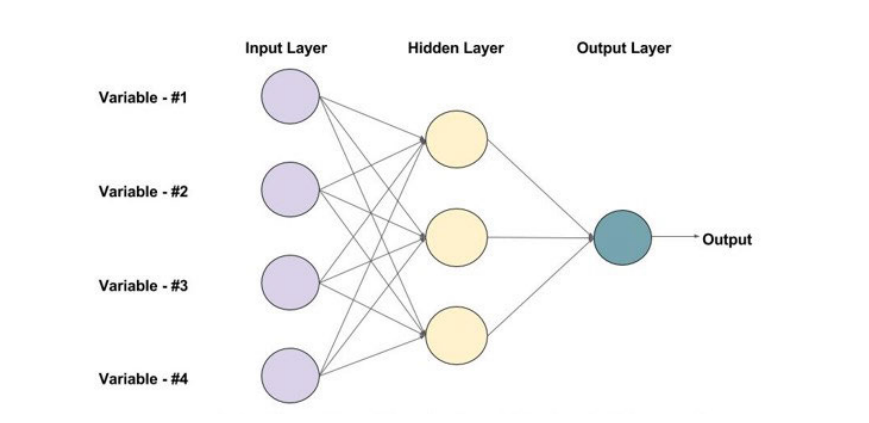
\includegraphics[width=0.75\textwidth]{fnn.png}
    \caption{Architecture of the Feedforward Neural Network}
    \label{fig:fnn}
\end{figure}

\section{Deep Neural Network}

A Deep Neural Network (DNN) extends the basic neural network
structure by using multiple layers of interconnected neurons. The
additional layers allow the model to learn increasingly complex
representations of the input data.

In the research, the DNN uses multiple fully connected layers with
ReLU activation functions and a sigmoid output unit. During
training, the network adjusts its parameters according to the
classification error so that it can distinguish between legitimate
and phishing instances.


\begin{figure}[H]
    \centering
    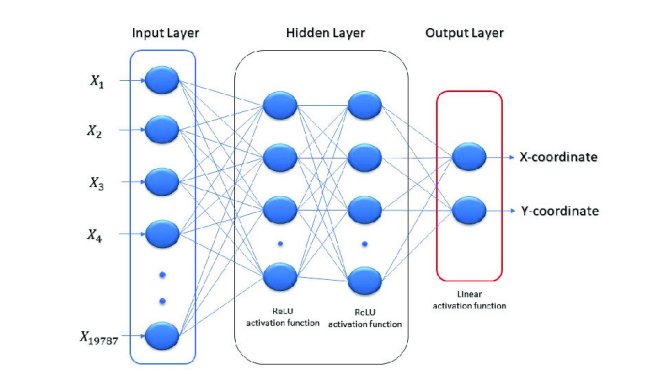
\includegraphics[width=0.75\textwidth]{dnn.png}
    \caption{Architecture of the Deep Neural Network}
    \label{fig:dnn}
\end{figure}
\section{Wide and Deep Model}

The Wide and Deep Model combines two different learning components:
a wide component and a deep component. The purpose of combining
these components is to utilize their complementary strengths.

The wide component is intended to capture and memorize specific
patterns in the input data, while the deep component learns more
complex patterns and generalizations through multiple neural
network layers. Combining these components allows the model to use
both memorization and generalization when performing classification.

The research implements the Wide and Deep Model using the functional
API of TensorFlow Keras. The model is evaluated as one of the four
deep learning approaches used for phishing detection.
\begin{figure}[H]
    \centering
    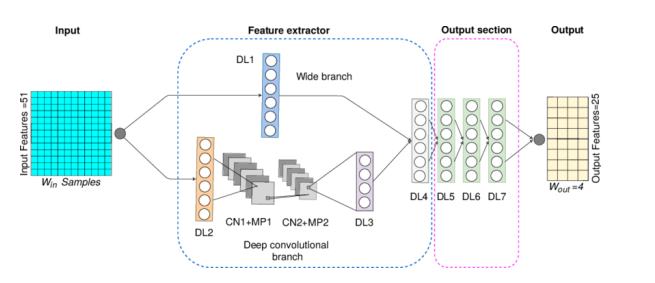
\includegraphics[width=0.85\textwidth]{widendeep.png}
    \caption{Architecture of the Wide and Deep Model}
    \label{fig:wide_deep}
\end{figure}

\section{TabNet}

TabNet is a deep learning architecture designed specifically for
tabular data. The model uses a sequential attention mechanism to
identify informative features during the decision-making process.

Instead of treating every input feature identically at every stage,
TabNet uses attention to determine which features are most useful
for the current decision step. This allows the model to focus on
informative portions of the input data and provides a mechanism for
feature selection within the learning process.

In the research, the TabNet model is initially trained using a
TabNetPretrainer and is subsequently fine-tuned for the
classification task. The model is therefore included alongside FNN,
DNN, and Wide and Deep to evaluate different deep learning
architectures for phishing detection.
\begin{figure}[H]
    \centering
    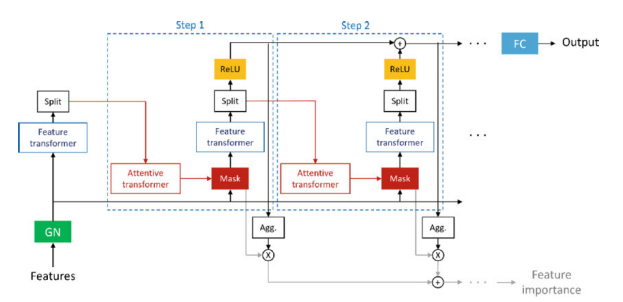
\includegraphics[width=0.85\textwidth]{tab.png}
    \caption{Architecture of the TabNet Model}
    \label{fig:tabnet}
\end{figure}
\section{Feature Selection}

Feature selection is the process of identifying the most relevant
features from a larger collection of available attributes. A
dataset may contain redundant, irrelevant, or less informative
features, and using all of them can increase computational
requirements.

For phishing detection, feature selection is particularly important
because the objective is not only to obtain accurate predictions but
also to develop a model that can evaluate URLs efficiently.
Reducing the number of features can decrease computational
complexity, reduce latency, and improve the practicality of a
detection system.

The research initially considers a large feature set and applies
preprocessing and feature-selection procedures before model
training. The dataset is subsequently reduced to 73 features, from
which the most relevant features are identified.

\section{Permutation Importance}

Permutation Importance is a model-agnostic technique used to
estimate the importance of individual features. The method evaluates
a feature by randomly shuffling its values and observing the change
in the model's performance.

If randomly permuting a feature produces a significant reduction in
model performance, that feature is considered important because the
model relies on it when making predictions. Conversely, a small
change in performance indicates that the feature has a smaller
contribution to the model.

In the research, Permutation Importance is applied to the FNN, DNN,
TabNet, and Wide and Deep models. The importance scores obtained
from the models are analyzed and used to rank the features. The
resulting ranking is then used to identify the most relevant
features for phishing detection.

The study reports that features such as
\texttt{qty\_slash\_url}, \texttt{time\_domain\_activation},
\texttt{length\_url}, \texttt{qty\_mx\_servers}, and
\texttt{tls\_ssl\_certificate} were among the highly ranked
features.

Permutation Importance is useful in this context because it
evaluates a feature according to its effect on actual model
performance. The research also compares its results with
Information Gain, Chi-Square, and Fisher's Score. The paper
highlights that these statistical methods are primarily univariate,
whereas Permutation Importance can evaluate feature contributions
within the context of the trained model.

\section{Data Preprocessing}

Data preprocessing prepares the collected data for machine learning
and helps maintain consistency during model training. In the
research, preprocessing includes handling single-valued columns,
identifying defective two-valued columns where one value is $-1$,
handling missing values, and applying Min-Max normalization.

Min-Max normalization rescales numerical feature values to a common
range. This helps prevent features with larger numerical scales from
having an inappropriate influence during model training.

After preprocessing, the resulting dataset provides a cleaner and
more consistent input representation for feature selection and
deep learning.

\section{Model Training and Cross-Validation}

After feature selection, the selected features are supplied to the
deep learning models for training and testing. The research uses
10-fold cross-validation to evaluate the models.

In 10-fold cross-validation, the dataset is divided into ten
subsets. The model is trained using nine subsets and evaluated using
the remaining subset. This process is repeated until every subset
has been used for evaluation. The results from the different folds
provide a more reliable estimate of model performance.

The research also uses stratified sampling so that the distribution
of legitimate and phishing instances remains representative across
the different folds. This reduces the possibility that an individual
fold becomes disproportionately dominated by one class.

\section{Model Evaluation}

Model evaluation determines how effectively a trained model
classifies phishing and legitimate instances. The research considers
several performance measures rather than relying only on accuracy.

\subsection{Accuracy}

Accuracy represents the proportion of correctly classified instances
among all evaluated instances. It provides a general measure of the
correctness of the classification model.

\begin{equation}
Accuracy =
\frac{TP + TN}{TP + TN + FP + FN}
\end{equation}

where $TP$ represents true positives, $TN$ represents true
negatives, $FP$ represents false positives, and $FN$ represents
false negatives.

\subsection{True Positive Rate}

True Positive Rate (TPR), also referred to as sensitivity or recall,
measures the proportion of actual phishing instances that are
correctly identified by the model.

\begin{equation}
TPR =
\frac{TP}{TP + FN}
\end{equation}

A high TPR is desirable in phishing detection because failing to
identify an actual phishing URL can expose a user to a malicious
website.

\subsection{False Positive Rate}

False Positive Rate (FPR) represents the proportion of legitimate
instances that are incorrectly classified as phishing.

\begin{equation}
FPR =
\frac{FP}{FP + TN}
\end{equation}

A low FPR is important because incorrectly blocking legitimate
websites can negatively affect the user experience.

\subsection{Testing Time}

Testing time measures the time required by a trained model to
process and classify test instances. This measure is particularly
relevant to phishing detection because practical systems may need to
evaluate URLs rapidly.

\subsection{Anti-Phishing Score}

The research introduces an anti-phishing score as a combined
performance measure. It considers accuracy, false positive rate,
true positive rate, and testing time to provide a broader assessment
of the phishing detection models.

The score is defined in the research as:

\begin{equation}
APS =
0.3 \times Accuracy
+ 0.25 \times (1-FPR)
+ 0.25 \times TPR
+ 0.2 \times TestingTime
\end{equation}

The testing-time component is treated according to the paper's
normalization/inverse-time approach so that faster testing
contributes positively to the overall score. Therefore, the formula
should not be interpreted as adding raw testing time directly.

The use of this combined measure allows the research to consider
both classification quality and practical detection efficiency when
comparing the different models.

%=========================================================
% CHAPTER 3
%=========================================================

\chapter{Literature Survey}

\section{Existing Phishing Detection Techniques}

Phishing is one of the major cybersecurity threats in which attackers attempt to deceive users by directing them to fraudulent websites or URLs that resemble legitimate services. Traditional phishing detection methods mainly include blacklist-based, heuristic, and rule-based approaches. Blacklist-based systems identify phishing websites by comparing a given URL with a database of previously reported malicious websites. Although this approach is effective for known phishing websites, it may fail to detect newly created or modified phishing URLs that have not yet been added to the blacklist.

Heuristic-based techniques attempt to identify suspicious characteristics in URLs or webpages. These characteristics may include unusual URL length, excessive use of special characters, suspicious domain information, and other structural properties. Such methods can detect previously unknown threats to some extent, but their effectiveness depends on the rules and characteristics selected by the system.

The rapidly changing nature of phishing attacks creates a need for more adaptive detection methods. Attackers continuously modify domains, URLs, and website structures to avoid existing detection mechanisms. This has encouraged researchers to investigate machine learning and deep learning techniques that can learn patterns directly from phishing and legitimate website data.

\section{Machine Learning Based Phishing Detection}

Machine learning provides a data-driven approach to phishing detection. Instead of depending entirely on predefined rules, machine learning models learn patterns from labelled datasets containing legitimate and phishing examples. Once trained, these models can classify previously unseen URLs based on the characteristics learned during training.

Different types of features can be used for phishing detection, including URL-based features, domain-related features, webpage characteristics, and other network-related information. URL-based features are particularly useful because they can be extracted from the URL itself without requiring extensive interaction with the webpage.

A URL contains several structural components that can provide useful information for classification. Features related to URL length, the number of directories, special characters, domain properties, and security-related characteristics can help distinguish phishing URLs from legitimate URLs. Machine learning models can learn relationships between these features and the corresponding class labels.

However, phishing datasets may contain a large number of features, and not all of them contribute equally to classification. Irrelevant or redundant features can increase computational requirements and may affect model performance. Therefore, feature selection is an important step in developing an efficient phishing detection system.

The use of machine learning also provides an opportunity to evaluate different models using common performance measures such as accuracy, true positive rate, false positive rate, and testing time. Such evaluation helps determine not only how accurately a model detects phishing URLs but also whether it is suitable for practical use.

\section{Deep Learning Based Phishing Detection}

Deep learning is an extension of machine learning that uses neural networks with multiple layers to learn complex patterns from data. Deep learning models have been increasingly investigated for cybersecurity applications because they can learn relationships between multiple input features and classification outcomes.

In phishing detection, deep learning can be applied to structured URL features. The study considered four different deep learning architectures: Feedforward Neural Network (FNN), Deep Neural Network (DNN), Wide and Deep Model, and TabNet.

The Feedforward Neural Network is a fully connected neural network in which information moves from the input layer through hidden layers to the output layer. In the selected study, ReLU activation is used in the hidden layers and a sigmoid function is used in the output layer for binary classification.

The Deep Neural Network uses multiple hidden layers to learn more complex relationships between the input features. Increasing the depth of the network allows it to represent more complicated patterns in the data.

The Wide and Deep Model combines a wide component with a deep component. The wide component is intended to capture direct feature relationships, while the deep component learns more complex patterns. This combination provides both memorization and generalization capabilities.

TabNet is a deep learning architecture designed for tabular data. It uses an attention mechanism to select relevant features during different decision steps. This allows the model to focus on informative parts of the input while performing classification.

The comparison of these four architectures allows the study to examine which model provides the most suitable balance between detection performance and practical efficiency.

\section{Feature Selection in Phishing Detection}

Feature selection is the process of selecting the most relevant features from a dataset while removing features that provide limited or redundant information. It is particularly important in phishing detection because URL datasets can contain a large number of characteristics.

Several feature-selection techniques have been used in related studies. Information Gain measures the reduction in uncertainty obtained from a feature, while Chi-Square evaluates the relationship between categorical features and class labels. Fisher's Score is another statistical method used to measure the ability of a feature to distinguish between different classes.

The selected study investigates Permutation Importance for feature selection. Permutation Importance evaluates the contribution of a feature by randomly changing its values and observing the effect on model performance. If shuffling a feature causes a significant reduction in performance, the feature is considered important to the model.

One advantage of Permutation Importance is that it evaluates feature contribution in the context of the trained model. Therefore, it can provide information about how features contribute to the predictive performance of different deep learning architectures.

In the study, feature selection was applied to the phishing dataset before model evaluation. Important URL-related features identified by the analysis include \texttt{qty\_slash\_url}, \texttt{time\_domain\_activation}, \texttt{length\_url}, \texttt{qty\_mx\_servers}, and \texttt{tls\_ssl\_certificate}. The feature-selection process helped reduce the dataset and provided a more focused set of inputs for the classification models.

\section{Research Gap}

Existing phishing detection techniques have demonstrated the usefulness of machine learning and deep learning for identifying malicious URLs. However, several challenges remain. Traditional blacklist-based approaches have difficulty identifying newly created phishing websites, while rule-based methods require continuous modification as attack techniques change.

Deep learning models can provide strong classification performance, but their effectiveness can depend on the quality and number of input features. Using unnecessary or redundant features can increase computational requirements and may reduce the efficiency of the detection system. Therefore, an appropriate feature-selection method is important for developing an effective model.

Another challenge is determining which deep learning architecture is most suitable for phishing URL classification. Different architectures may provide different levels of accuracy, computational cost, and generalization capability. Evaluating several models under the same experimental conditions can provide a better basis for model selection.

The selected study addresses these gaps by combining URL-based feature extraction, preprocessing, feature selection using Permutation Importance, and multiple deep learning architectures. FNN, DNN, Wide and Deep, and TabNet are evaluated using selected features. The models are compared using performance measures including accuracy, false positive rate, true positive rate, testing time, and an anti-phishing score. The study also uses a second dataset to examine the selected model on new data.

Thus, the work focuses not only on achieving high phishing detection accuracy but also on identifying an efficient feature set and a suitable deep learning model for practical phishing detection.

%=========================================================
% CHAPTER 4
%=========================================================

\chapter{Proposed Methodology}

\section{Overview of the Proposed Method}

The proposed system is designed to detect phishing URLs using machine learning and deep learning techniques. The overall process consists of dataset preparation, URL feature extraction, data preprocessing, feature selection, model training, and performance evaluation. Four deep learning models, namely Feedforward Neural Network (FNN), Deep Neural Network (DNN), Wide and Deep Model, and TabNet, are evaluated for phishing classification.

The methodology begins with a labelled phishing URL dataset. Features are extracted from the URL components and the resulting data is preprocessed before being provided to the classification models. Permutation Importance is then used to identify important features and reduce the feature set. The selected features are used to train and evaluate the deep learning models using cross-validation.

\begin{figure}[H]
    \centering
    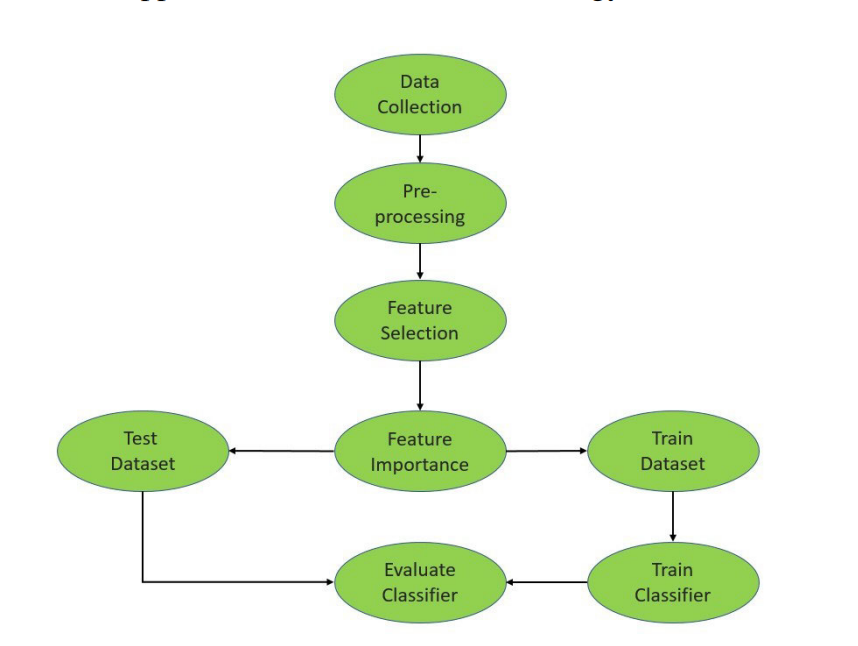
\includegraphics[width=0.82\textwidth]{figures/methodology.png}
    \caption{Overview of the proposed phishing detection methodology}
    \label{fig:methodology}
\end{figure}

\section{Dataset and Data Collection}

The primary dataset used in the study is the Mendeley phishing URL dataset published in 2020. The dataset contains URLs classified into two categories: legitimate and phishing. The class label is represented by the \texttt{phishing} attribute, where 0 represents a legitimate URL and 1 represents a phishing URL.

A second dataset published in 2021 is used to validate the selected model. In this dataset, the class is represented by the \texttt{status} attribute, containing the values \texttt{legitimate} and \texttt{phishing}. The use of a separate dataset provides an additional evaluation of the model's ability to classify previously unseen data.

The experiments are implemented using Python along with TensorFlow and Keras for developing the deep learning models.

\section{URL Feature Extraction}

URLs contain structural information that can be used to identify suspicious websites. The study extracts features from different components of URLs, including the domain, directory, file, and parameters.

\begin{figure}[H]
    \centering
    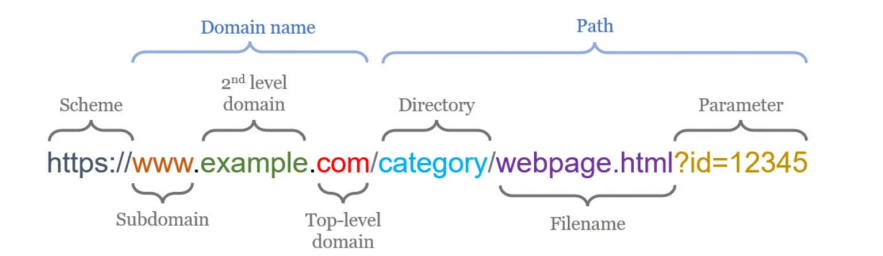
\includegraphics[width=0.72\textwidth]{figures/url_structure.png}
    \caption{Basic structure of a URL}
    \label{fig:urlstructure}
\end{figure}

The URL is divided into its major components and characteristics are calculated from these components. A total of 17 URL-structure-related features are generated from the URL components in the dataset. These features describe characteristics such as URL length, the number of slashes, domain properties, and other structural information.

The extracted features provide the input variables required by the classification models. Since phishing URLs often contain structural characteristics that differ from legitimate URLs, these features can provide useful information for distinguishing the two classes.

\section{Data Preprocessing}

Before training the models, the collected data is preprocessed to ensure that the input features are suitable for machine learning. Columns containing a single value are removed because they do not provide useful information for classification. Defective two-valued columns in which one value is represented by $-1$ are also handled during preprocessing.

Missing values are addressed before model training. The numerical features are then normalized using Min-Max normalization so that the input variables are brought to a common scale.

The preprocessing stage helps improve the consistency of the dataset and prevents features with larger numerical ranges from having an unnecessary influence on the learning process.

\section{Feature Selection Using Permutation Importance}

After preprocessing, feature selection is performed to identify the features that contribute most to phishing classification. The primary technique used is Permutation Importance.

In this method, the values of one feature are randomly shuffled while the other features remain unchanged. The trained model is then evaluated to determine how much its performance changes. A large decrease in performance indicates that the feature has an important contribution to the model.

Permutation Importance is applied to the different deep learning models used in the study. The resulting importance values are used to rank the features and select the most relevant ones.

\begin{figure}[H]
    \centering
    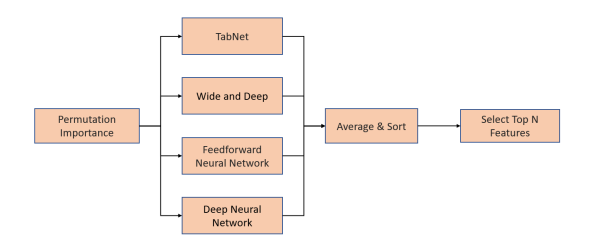
\includegraphics[width=0.75\textwidth]{figures/permutation_importance.png}
    \caption{Feature selection using Permutation Importance}
    \label{fig:permutation}
\end{figure}

The study also compares Permutation Importance with Information Gain, Chi-Square, and Fisher's Score. These comparisons are used to examine the effectiveness of different feature-selection approaches. The selected features include important URL characteristics such as \texttt{qty\_slash\_url}, \texttt{time\_domain\_activation}, \texttt{length\_url}, \texttt{qty\_mx\_servers}, and \texttt{tls\_ssl\_certificate}.

\section{Deep Learning Models}

Four deep learning models are considered in the proposed system.

\subsection{Feedforward Neural Network}

The Feedforward Neural Network consists of an input layer, fully connected hidden layers, and an output layer. ReLU activation is used in the hidden layers, while the output layer uses a sigmoid activation function for binary classification.

The FNN learns a mapping between the selected URL features and the phishing or legitimate class. Its relatively straightforward architecture also makes it suitable for efficient classification.

\subsection{Deep Neural Network}

The Deep Neural Network uses multiple fully connected hidden layers to learn more complex relationships between the input features. Similar to the FNN, ReLU activation is used in the hidden layers and sigmoid activation is used for the final binary prediction.

The additional depth allows the model to learn higher-level representations of the input features.

\subsection{Wide and Deep Model}

The Wide and Deep Model combines two learning components. The wide component is responsible for learning direct feature relationships, while the deep component learns more complex patterns through multiple neural-network layers.

This combination allows the model to use both memorization and generalization during classification.

\subsection{TabNet}

TabNet is designed for classification tasks involving tabular data. It uses sequential attention to determine which features should receive more attention during different decision steps.

In the study, TabNet is first pretrained using a TabNet pretrainer and is subsequently fine-tuned for the phishing classification task. This allows the model to learn useful representations from the tabular URL features.

\section{Model Training and Evaluation}

The selected features are provided to the four deep learning models for training and classification. The study uses 10-fold cross-validation with stratified sampling to evaluate the models. In this approach, the dataset is divided into ten subsets, with the class distribution maintained across the folds.

The models are evaluated using accuracy, True Positive Rate (TPR), False Positive Rate (FPR), and testing time. ROC and Precision-Recall curves are also used to compare the classification performance of the models.

Hyperparameter optimization is performed using grid search. Parameters such as the number of selected features, training iterations, batch size, dropout, and other training settings are considered during model optimization.

\section{Model Selection}

The final model is selected by considering both predictive performance and computational efficiency. Although obtaining high classification accuracy is important, a phishing detection system must also be capable of making predictions efficiently.

The study further evaluates the selected configuration using a second dataset. This provides an additional indication of the model's generalization capability and practical suitability for phishing detection.

The complete methodology therefore combines URL-based feature extraction, preprocessing, Permutation Importance, deep learning classification, cross-validation, and hyperparameter optimization to develop an effective phishing detection system.

%=========================================================
% CHAPTER 5
%=========================================================

\chapter{Results and Discussion}

\section{Feature Selection Results}

The feature-selection stage was used to identify the URL features that contribute most to phishing classification. Permutation Importance was applied to the trained models to determine the effect of individual features on model performance.

After preprocessing and feature selection, the dataset was reduced to a more manageable feature set. Among the important features identified were \texttt{qty\_slash\_url}, \texttt{time\_domain\_activation}, \texttt{length\_url}, \texttt{qty\_mx\_servers}, and \texttt{tls\_ssl\_certificate}. These features describe different characteristics of the URL and domain and provide useful information for distinguishing phishing URLs from legitimate URLs.

The study also compared Permutation Importance with Information Gain, Chi-Square, and Fisher's Score. These methods produced different feature rankings. Permutation Importance was particularly useful because it evaluates the effect of a feature on the performance of the trained model rather than considering the feature independently of the model.

\section{Model Performance}

The four deep learning models, namely FNN, DNN, Wide and Deep, and TabNet, were evaluated using the selected features. Ten-fold cross-validation with stratified sampling was used during evaluation.

The models were compared using accuracy, True Positive Rate (TPR), False Positive Rate (FPR), testing time, and the Anti-Phishing Score. These measures provide information about both the classification capability and practical efficiency of each model.

\begin{table}[H]
\centering
\caption{Comparison of Deep Learning Models}
\label{tab:modelcomparison}
\begin{tabular}{lcc}
\toprule
\textbf{Model} & \textbf{AUC} & \textbf{Anti-Phishing Score} \\
\midrule
FNN & 0.99 & 0.9521 \\
DNN & 0.98 & 0.7479 \\
Wide and Deep & 0.98 &0.8788 \\
TabNet & 0.97 & 0.7420 \\
\bottomrule
\end{tabular}
\end{table}

The FNN achieved the highest AUC of 0.99, followed by DNN and Wide and Deep with an AUC of 0.98. TabNet achieved an AUC of 0.97. The results indicate that all four models were capable of distinguishing phishing URLs from legitimate URLs, while the FNN provided the strongest overall discrimination among the evaluated models.

\section{ROC and Precision-Recall Analysis}

Receiver Operating Characteristic (ROC) curves were used to analyze the classification performance of the models at different classification thresholds. The Area Under the Curve (AUC) provides a measure of the model's ability to distinguish between phishing and legitimate URLs.

\begin{figure}[H]
    \centering
    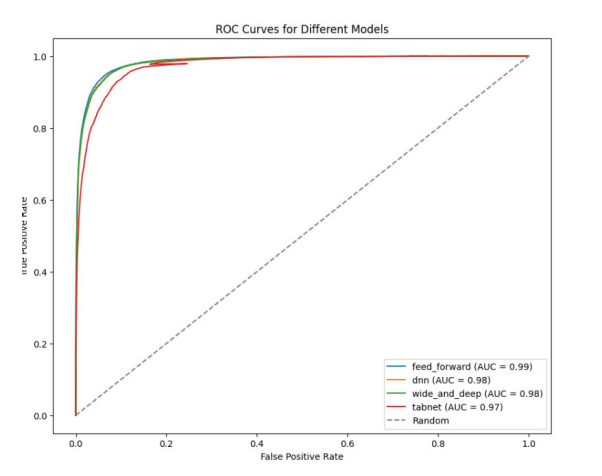
\includegraphics[width=0.78\textwidth]{figures/roc_curves.png}
    \caption{ROC curves of the evaluated deep learning models}
    \label{fig:roc}
\end{figure}

The FNN produced the highest AUC value of 0.99, indicating strong classification capability. DNN and Wide and Deep achieved an AUC of 0.98, while TabNet achieved 0.97.

Precision-Recall curves were also considered because they provide useful information about classification performance, particularly when identifying positive phishing instances.

\begin{figure}[H]
    \centering
    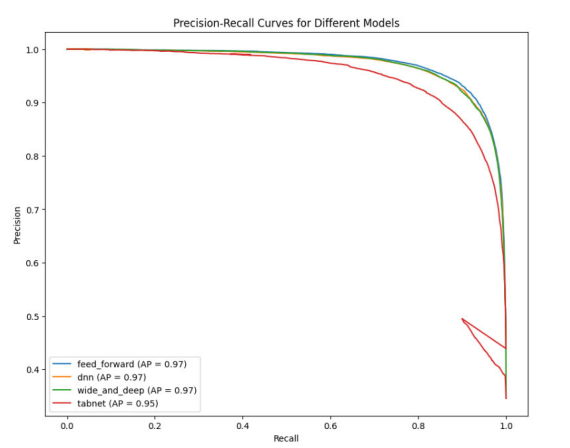
\includegraphics[width=0.78\textwidth]{figures/pr_curves.png}
    \caption{Precision-Recall curves of the evaluated models}
    \label{fig:pr}
\end{figure}

The ROC and Precision-Recall analyses demonstrate that the evaluated models can effectively separate phishing URLs from legitimate URLs. The results also support the selection of FNN as the strongest performing model among the four architectures.

\section{Anti-Phishing Score}

In addition to individual evaluation metrics, the study uses an Anti-Phishing Score to provide a combined measure of model performance. The score considers accuracy, false positive rate, true positive rate, and testing time.

The Anti-Phishing Score is calculated using weighted contributions from these performance measures:

\begin{equation}
APS =
0.3 \times Accuracy
+ 0.25 \times (1-FPR)
+ 0.25 \times TPR
+ 0.2 \times TestingTime
\end{equation}

The testing-time component is normalized or represented as an inverse-time measure so that better testing efficiency contributes positively to the overall score.

The FNN achieved an Anti-Phishing Score of \textbf{0.9521}. This result, together with its high AUC, supports the selection of FNN as the most suitable model in the study.

\section{Hyperparameter Optimization}

Grid search was used to investigate different model configurations and identify a suitable combination of selected features and training iterations. The results showed that a configuration using 20 features and 40 training iterations achieved an accuracy of approximately \textbf{95.53\%}.

However, the study selected a configuration using 14 features and 50 training iterations for practical use. This configuration achieved an accuracy of approximately \textbf{94.46\%} while requiring lower computational resources.

The difference between the two configurations demonstrates that the highest accuracy is not necessarily the only factor considered when selecting a practical phishing detection model. Computational efficiency is also important, particularly when the model is intended for real-time detection.

\section{Validation Using a Second Dataset}

The selected model was further evaluated using a second phishing dataset published in 2021. This dataset uses the \texttt{status} attribute to identify URLs as either legitimate or phishing.

When tested on the second dataset, the selected model achieved an accuracy of approximately \textbf{80\%}. Although this performance was lower than the result obtained on the primary dataset, the experiment provides evidence about the model's ability to classify data from a different source.

The decrease in accuracy also highlights the difficulty of maintaining performance when phishing data changes over time. This is an important consideration for practical phishing detection systems because new phishing techniques and URL structures can differ from those present in the training data.

\section{Discussion}

The experimental results demonstrate that combining feature selection with deep learning can provide an effective approach to phishing URL detection. The use of Permutation Importance helps identify relevant features, while the comparison of different deep learning architectures provides a basis for selecting an appropriate classification model.

Among the four evaluated architectures, FNN produced the highest AUC and Anti-Phishing Score. The grid-search results also show that a slightly lower accuracy configuration can be preferable when it provides reduced computational requirements.

The evaluation using a second dataset demonstrates that generalization remains an important challenge. The reduction in accuracy on new data indicates that phishing detection models should be continuously evaluated and updated as attack patterns evolve.

Overall, the results indicate that the FNN-based configuration provides a suitable balance between detection performance and computational efficiency, making it the preferred model for the practical phishing detection system described in the study.

%=========================================================
% CHAPTER 6
%=========================================================

\chapter{Applications and Practical Implementation}

\section{Automated Phishing URL Detection}

The proposed phishing detection system can be used to automatically classify URLs as either legitimate or phishing. Instead of relying only on manually maintained blacklists, the system uses URL-based features and a trained deep learning model to identify suspicious patterns.

The selected FNN model provides a practical solution because it achieved strong classification performance while maintaining comparatively low computational requirements. The use of a reduced feature set also helps decrease the amount of information that needs to be processed during prediction.

Automated classification can be useful in environments where a large number of URLs need to be analyzed. The system can process URLs and provide a classification result without requiring a user to manually inspect the website.

\section{Browser-Based Phishing Prevention}

One practical application described in the study is a phishing-prevention browser extension. The extension is designed to obtain the URL accessed by the user and send it to a Flask server for classification.


The browser extension uses web crawling to extract the URL and communicates with the server containing the machine learning model. The server processes the URL and determines whether it is harmful. Based on the classification result, the system can help prevent users from accessing potentially malicious websites.

This type of implementation provides a direct connection between the trained machine learning model and an end-user security application.

\section{Real-Time Phishing Prevention}

Phishing detection systems are particularly useful when they can provide results quickly. A delay in classification can reduce the usefulness of a security system because users may already have interacted with a malicious website.

The proposed approach considers testing time along with classification accuracy, true positive rate, and false positive rate. Feature selection further contributes to computational efficiency by reducing the number of input variables used by the model.

The selected model configuration provides a balance between detection performance and computational requirements. This makes the approach suitable for applications where URLs need to be evaluated rapidly.

\section{Integration With Security Systems}

The phishing detection approach can also be extended beyond browser-based applications. A trained phishing classifier can potentially be integrated with other cybersecurity systems to provide an additional layer of URL-based threat detection.

The study identifies integration with Network Intrusion Detection Systems (NIDS) and endpoint protection systems as possible future applications. Such integration could allow suspicious URLs to be analyzed as part of a larger security-monitoring framework.

Threat-intelligence sharing can also improve the effectiveness of phishing detection. Information obtained from detected phishing URLs can be used to support other security components and help identify emerging threats.

\section{Practical Limitations}

Although the proposed system provides effective phishing classification, its performance can vary when applied to new datasets. The evaluation using a second dataset resulted in an accuracy of approximately 80\%, compared with the higher accuracy obtained on the primary dataset.

This difference indicates that phishing detection models may be affected by changes in URL structures and attack patterns. Therefore, models intended for real-world deployment should be periodically evaluated and updated using recent phishing data.

Another consideration is the possibility of adversarial manipulation. Attackers may modify URL characteristics to make phishing URLs appear more similar to legitimate URLs. Improving the robustness of the model against such attacks is therefore an important area for future development.

\section{Future Scope}

The study identifies several possible directions for future development. The phishing detection system can be integrated with NIDS and endpoint protection solutions to provide broader security coverage.

Threat-intelligence sharing can also be incorporated to improve the identification of newly emerging phishing attacks. Further research can investigate the robustness of the models against adversarial machine-learning techniques.

The browser extension can also be improved to provide faster detection and a more effective user-warning mechanism. Continuous training with updated phishing datasets can further improve the ability of the system to adapt to changing attack patterns.

%=========================================================
% CHAPTER 7
%=========================================================

\chapter{Conclusion and Future Scope}

\section{Conclusion}

Phishing continues to be a significant cybersecurity threat because attackers constantly create new fraudulent websites and modify existing attack techniques. Traditional approaches such as blacklists and manually defined rules have limitations when dealing with newly generated phishing URLs. Machine learning and deep learning provide a more adaptive approach by learning patterns from URL-based features.

The study investigated a machine learning approach for phishing detection by combining feature selection with deep learning models. URL-related features were extracted and preprocessed before being used for classification. Permutation Importance was applied to identify features that contributed significantly to model performance and to reduce the feature set.

Four deep learning architectures---Feedforward Neural Network (FNN), Deep Neural Network (DNN), Wide and Deep Model, and TabNet---were evaluated. The models were compared using accuracy, True Positive Rate, False Positive Rate, testing time, ROC analysis, Precision-Recall analysis, and the Anti-Phishing Score.

Among the evaluated models, the FNN achieved the highest AUC of 0.99 and an Anti-Phishing Score of 0.9521. The study also used grid search to investigate different feature and training configurations. Although a configuration using 20 features and 40 iterations achieved 95.53\% accuracy, a configuration using 14 features and 50 iterations was selected for practical use, achieving 94.46\% accuracy with lower computational requirements.

The selected model was further evaluated using a second dataset, where it achieved approximately 80\% accuracy. This result demonstrates the importance of testing phishing detection models on new data, since changes in phishing techniques and URL structures can affect model performance.

Overall, the study demonstrates that combining effective feature selection with deep learning can provide a useful approach for phishing URL detection. The FNN was identified as the most suitable model among the evaluated architectures because of its strong classification performance and practical efficiency. The development of a browser extension connected to a Flask-based classification server further demonstrates the potential for applying the model in a practical phishing-prevention system.

\section{Future Scope}

The proposed phishing detection system can be further improved in several directions. Integration with Network Intrusion Detection Systems (NIDS) and endpoint protection platforms could extend the use of the model beyond browser-based detection.

Another important direction is the integration of threat-intelligence sharing. Information about newly detected phishing URLs can be used to improve detection and support other security systems.

Future research can also focus on improving the robustness of the model against adversarial machine-learning techniques. Attackers may modify URL characteristics in an attempt to bypass machine learning-based detection, making adversarial robustness an important consideration for real-world deployment.

The browser extension can be further improved to provide faster detection, better user warnings, and more efficient communication with the classification server. Finally, regularly updating the training data with newly identified phishing URLs can help the model adapt to changing attack patterns and improve its generalization to emerging threats.

%=========================================================
% REFERENCES
%=========================================================

\chapter*{References}
\addcontentsline{toc}{chapter}{References}

\begin{enumerate}

\item F. Salahdine, Z. E. Mrabet, and N. Kaabouch,
``Phishing attacks detection a machine learning-based approach,''
in \textit{Proc. IEEE 12th Annu. Ubiquitous Comput., Electron. Mobile
Commun. Conf. (UEMCON)}, New York, NY, USA, Dec. 2021, pp. 250--255.

\item M. Baykara and Z. Z. G\"urel,
``Detection of phishing attacks,''
in \textit{Proc. 6th Int. Symp. Digit. Forensic Secur. (ISDFS)},
Antalya, Turkey, Mar. 2018, pp. 1--5.

\item K. L. Chiew, K. S. C. Yong, and C. L. Tan,
``A survey of phishing attacks: Their types, vectors and technical approaches,''
\textit{Expert Syst. Appl.}, vol. 106, pp. 1--20, Sep. 2018.

\item F. Yahya,
``Detection of phishing websites using machine learning approaches,''
in \textit{Proc. Int. Conf. Data Sci. Appl. (ICoDSA)},
Bandung, Indonesia, 2021, pp. 40--47.

\item A. Alswailem, B. Alabdullah, N. Alrumayh, and A. Alsedrani,
``Detecting phishing websites using machine learning,''
in \textit{Proc. 2nd Int. Conf. Comput. Appl. Inf. Secur. (ICCAIS)},
Riyadh, Saudi Arabia, May 2019, pp. 1--6.

\item H. Zuhair, A. Selamat, and M. Salleh,
``Feature selection for phishing detection: A review of research,''
\textit{Int. J. Intell. Syst. Technol. Appl.}, vol. 15, no. 2, p. 147, 2016.

\item Mendeley Data. (Sep. 2020).
\textit{Phishing Websites Dataset}. [Online].
Available: \url{https://data.mendeley.com/datasets/72ptz43s9v/1}

\item Mendeley Data. (2021).
\textit{Web Page Phishing Detection Dataset}. [Online].
Available: \url{https://data.mendeley.com/datasets/c2gw7fy2j4/3}

\item P. Chinnasamy, N. Kumaresan, R. Selvaraj, S. Dhanasekaran,
K. Ramprathap, and S. Boddu,
``An efficient phishing attack detection using machine learning algorithms,''
in \textit{Proc. Int. Conf. Advancements Smart, Secure Intell. Comput. (ASSIC)},
Bhubaneswar, India, Nov. 2022, pp. 1--6.

\item T. Rincy N and R. Gupta,
``Feature selection techniques and its importance in machine learning: A survey,''
in \textit{Proc. IEEE Int. Students' Conf. Elect., Electron. Comput. Sci. (SCEECS)},
Bhopal, India, Feb. 2020, pp. 1--6.

\item R. Ramachandran, G. Ravichandran, and A. Raveendran,
``Evaluation of dimensionality reduction techniques for big data,''
in \textit{Proc. 4th Int. Conf. Comput. Methodologies Commun. (ICCMC)},
Erode, India, Mar. 2020, pp. 226--231.

\item S. Dangwal and A.-N. Moldovan,
``Feature selection for machine learning-based phishing websites detection,''
in \textit{Proc. Int. Conf. Cyber Situational Awareness, Data Anal. Assessment (CyberSA)},
Dublin, Ireland, Jun. 2021, pp. 1--6.

\item Y. Wei and Y. Sekiya,
``Feature selection approach for phishing detection based on machine learning,''
in \textit{Proc. Int. Conf. Appl. CyberSecur. (ACS)},
H. R. Hassen and H. Batatia, Eds., Cham, Switzerland: Springer, Jan. 2022,
pp. 61--70.

\item M. R. Chinguwo and R. Dhanalakshmi,
``Detecting cloud based phishing attacks using stacking ensemble machine learning technique,''
\textit{Int. J. Res. Appl. Sci. Eng. Technol.}, vol. 11, no. 3,
pp. 360--367, Mar. 2023, doi: 10.22214/ijraset.2023.49422.

\end{enumerate}%=========================================================
% END DOCUMENT
%=========================================================

\end{document}